
%Preambule

\documentclass {report}

% Import des extensions

\usepackage{hyperref}%pour insérer des liens
%\usepackage [francais]{minitoc}% permet de faire une table des matieres par chapitre
\usepackage  [francais,english]{babel} %il permet l'adaptation de LaTeX du français.
\usepackage [francais,nohints]{minitoc} % nohints permet d effacer l erreur des hints qu il y a quand on utilise les minitocs 
\setcounter{secnumdepth}{3}
%\setcounter{tocdepth}{2}
\setcounter{minitocdepth}{4}
\usepackage [T1]{fontenc} %il permet de spécifier à LaTeX l'utilisation du codage de caractères T1
\usepackage  [utf8]{inputenc} %gestion␣des␣accents␣
%\usepackage[latin1]{inputenc} %un package il permet d'utiliser les caractères ISO 8859-1

%\usepackage{listings} \lstset{ language=SQL, basicstyle=\small, numbers=left, numbersep=7pt, } %, numberstyle=\normalsize, 
%L'environnement  lstlisting L'environnement lstlisting permet de mettre en forme de façon colorée et d'utiliser de nombreuses options pour afficher du code.

\usepackage{verbatim} %L'environnement verbatim, accompagné du package du même nom, permet d'encadrer de gros volumes de code. Petit souci : il remplace les tabulations par des espaces.
%\usepackage{setspace}
\usepackage{parskip} % espace entre paragraphe
\usepackage{framed}
\usepackage{amssymb,amsmath,mathrsfs,mathtools}%package de math AMS et outils de math
\usepackage{color} % couleur
\usepackage{url}


%\usepackage[french]{minitoc}% permet de faire une table des matieres par chapitre
 %* Le package 'minitoc', disponible sur ftp://ftp.inria.fr/pub/TeX/CTAN/macros/latex/contrib/minitoc/, permet de construire une minitable des matières au début de chaque chapitre sous les classes 'book' et 'report'. Pour l'utiliser, il faut appeler les commandes \dominitoc avant la commande \tableofcontents habituelle. La commande \faketableofcontents permet de ne garder que les tables des matières locales et remplace alors la commande \tableofcontents. La commande \minitoc doit être appelée après chaque commande de début de chapitre \chapter dans lequel on veut inclure une table locale. A chaque appel de minitoc correspond un fichier .mtc<n> où n est le numéro du chapitre. Le compteur minitocdepth permet de fixer la profondeur des tables des matières désirées.

%\usepackage{lipsum}%Imprime du texte. Le paramètre optionnel permet de varier le texte imprimé.

\usepackage [pdftex]{graphicx} % gestion image
\usepackage [top=2cm,bottom=2cm,left=4cm,right=4cm] {geometry}%pour gérer les marges et dimension,la mise en page

%\usepackage{lastpage}%Il est possible de faire référence au nombre total de pages du document.  our obtenir un compteur de pages du type 1/3, 2/3, il faut charger dans le préambule du document le package lastpage.sty par la commande : usepackage{lastpage}Dans un champ de l’en-tête, il suffit alors d’insérer la commande :thepage/\pageref{LastPage}

%\usepackage[Sonny,Lenny]{fncychap} %Pour de beaux titres de chapitres dans vos documents, mettez dans le préambule \usepackage[Lenny]{fncychap} % Sonny, Lenny, Glenn, Conny, Rejne, Bjarne
%\usepackage{fancyhdr}%pour?les?en-têtes


% ajoute (entre autre) la bibliographie dans la table des matieres 
\usepackage[nottoc]{tocbibind}
\usepackage{natbib}
 
% biblio ordonnee classique
%\bibliographystyle{unsrt}
 

\usepackage{ragged2e} % justifie le texte

\hyphenation{intrusion}
\hyphenation{représente}
\hyphenation{automatique}
\hyphenation{exploration}
\hyphenation{construction}
\hyphenation{Utiliser}
\hyphenation{détection}
\hyphenation{outils}
\hyphenation{données}


%\usepackage{array}
%\usepackage{titlesec}%pour?les?sections
%\usepackage{titletoc}%pour?la?table?des?matières
%\usepackage{titling}%pour?le?

%\usepackage{hyperref}[pdftex]
%\usepackage[french]{varioref}

%\setcounter{secnumdepth}{1}
%\addto\captionsfrench{\renewcommand{\contentsname}{Sommaire}} %change le nom de la table de matieres

%fin 
%%%%%%%%%%%%%%%%%%%%%%%%%%%%%%%%%%%%%%%%%%%%%%%%%%%%%%%%%%%%%%%%%%%%%%%%%%%%%%%%%%%%%%




%%%%%%%%%%%%%%%%%%%%%%%%%%%%%%%%%%%%%%%%%%%%%%%%%%%%%%%%%%%%%%%%%%%%%%%%%%%%%%%%%%%%%%
%partie concernant la gestion des entêtes
%\pagestyle {fancy}
%\renewcommand\headrulewidth{2pt} %Ligne de séparation entre l'en-tête et le corps ,Pour forcer l’affichage d’une ligne horizontale, il suffit d’utiliser la commande \renewcommand{\headrulewidth}{1pt}, pour les en-têtes et \renewcommand{\footrulewidth}{1pt}, pour les pieds de page. détermine l'épaisseur du trait. Par défaut
%\renewcommand\headheight{2cm}

%\fancyhead[L]{\includegraphics [height=10mm,width=10mm] {ODM}} %haut de page gauche
%\fancyhead[R]{\includegraphics [height=10mm,width=10mm] {thumb-LOGO-UCAD}} %haut de page droite

%\fancyhead[C] {\leftmark}
%\fancyfoot[R]{\thepage/\pageref{LastPage}}

%\renewcommand\footrulewidth{2pt}%Ligne de séparation entre le corps et le pied de page,pour ne pas afficher de ligne horizontale, il suffit d’utiliser la commande \renewcommand{\headrulewidth}{0pt}, pour les en-têtes et \renewcommand{\footrulewidth}{0pt}, pour les pieds de page.
%\fancyfoot[C]{\thepage}
%\lfoot{Section \thesection}

%fin
%%%%%%%%%%%%%%%%%%%%%%%%%%%%%%%%%%%%%%%%%%%%%%%%%%%%%%%%%%%%%%%%%%%%%%%%%%%%%%%%%%%%%%




%%%%%%%%%%%%%%%%%%%%%%%%%%%%%%%%%%%%%%%%%%%%%%%%%%%%%%%%%%%%%%%%%%%%%%%%%%%%%%%%%%%%%%
%Redaction du document et enumerations des differentes parties 
%Corps du document
%Environnement

\begin{document}
% preparation des minitocs
\dominitoc
%\doparttoc

  %\dominitoc
	

\pagenumbering{roman} % numerote les page en chiffre romain 
% inclusion des chapitres
	

  %
%%%% Réalisation de la page de garde

\begin{titlepage}
\begin{center}
%\flushleft

\includegraphics[height=30mm,width=30mm]{logo.jpg} %insérer un dessin
\hfill%
%\hspace*{10,5cm}
%\includegraphics[height=30mm,width=30mm]{logo_gbi.jpg}\\
%\begin{center}
%\centering
%\includegraphics[height=20mm,width=20mm]{institut_limerick.jpg}
%\hspace*{1cm}
%\flushright

\includegraphics[height=40mm,width=20mm]{logo_sfa.jpg}\\
\end{center}
\vspace*{1cm}



%%%%%%%%%%%%%%%%%%% Déclaration du type de document%%%%%%%%%%%%%%%%%%%%%%%%%
\begin{center}
\textsc{Universit\'e de Poitiers,}\paragraph{}
 Master 1 Réseaux Télécommunications Multimédia et Automatique
\end{center}


\begin{center}
\texttt{Compte rendu de Travaux pratiques\\ Système de Transmission Multimedia}\\
\texttt{Du 26 Mars au 14 Avril 2015} %textcolor c est pour mettre la couleur 
\end{center}
\vspace*{2cm}
 



%\textsc{Universit\'e de Poitiers, M1 RTMA} \\ %[25pt] % Your university, school and/or department name(s)
%\horrule{0.5pt} \\[0.4cm] % Thin top horizontal rule
%\huge {\color{blue}Travaux pratiques en Méthodes statistiques}  % Title

%\author{Guy-Florent \textsc{Sadeler}, \\Thomas \textsc{Le Bris}.} % Author name

%\date{\today} % Date for the report \date{\normalsize\today} % Today's date or a custom date 
 
 
\begin{center}
%\begin{framed}
% Commande permettant de définir l'écart
\setlength{\fboxsep}{2mm}
% Commande permettant de définir l'épaisseur du trait
\setlength{\fboxrule}{2mm}
\fbox{\textcolor{blue}{{{\textbf{\textit{\fontfamily{pnc}\selectfont{Transmission Multimedia sur canaux extrêmement sensibles (Qualité et sécurité)}}}}}}}%textsc utiliser pour petite majuscule, \selectfont	active la police définie
%\end{framed}
\end{center}

\vspace*{1.5cm}
\begin{center}
\begin {figure}[htbp]
  \hbox{ 
     
\includegraphics[height=50mm,width=70mm]{intro2}%[width=5cm][scale=0.45]
     \hspace*{1cm}  %% pour mettre un espace (horizontal) de 5cm entre les deux images
     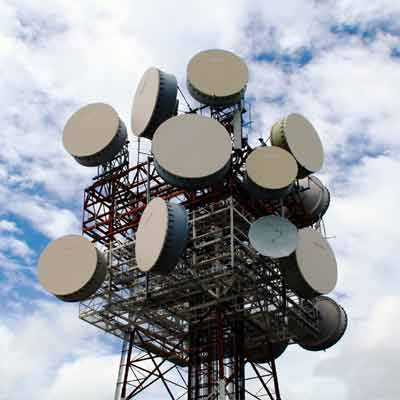
\includegraphics[height=50mm,width=70mm]{tel}
  }
\end {figure}
\end{center}


\vspace*{1cm}

%\par \vspace{2cm}
%\begin{center}
%\includegraphics[height=60mm,width=60mm]{gaussienne.jpg}
%\end{center}
%\par \vspace{2cm}


  % emphasize mettre l'accent sur le texte mis en accolade
 %textbf pour mettre le texte en gras 


\begin{center}
\begin{tabular}{l r}

Groupe d'étudiants: & \texttt{Guy-Florent \textsc{Sadeler} }\\ % Partner names
&  \texttt{Thomas \textsc{Le Bris}}

\end{tabular}
\end{center}

\vspace*{1cm}
\begin{center}
\begin{tabular}{l r}
Responsable pédagogique: & \texttt{Clency \textsc{Perrine}} % Instructor/supervisor
\end{tabular}
\end{center}




\end{titlepage}
	
	\newpage
	\null 
	\thispagestyle{empty}
	
	
	%\include{Rthanks}
	
	%\include{RabstractE}

	%\include{Rabstract}

	\tableofcontents %Insertion de lignes de pointillés avec dotfill

  %\setcounter{secnumdepth}{1}
	%\setcounter{tocdepth}{2} % On ajuste la profondeur


  %\selectlanguage {french}
	%\addcontentsline{toc}{chapter}{Table des Figures}
	\listoffigures
	
	%\selectlanguage {french}
	%\addcontentsline{toc}{chapter}{Liste des Tableaux}
	\listoftables

	%\include{Rquote}
	
	\pagenumbering{arabic}
	
	%\chapter*{Avant-propos}
%\addcontentsline{toc}{chapter}{Introduction}
%\minitoc

At the University of Poitiers, students in Master of Information and Communication Systems, Emphasis  (professional and research career) in NetworkTechnologies field have to carry out a project during their first year in order to complete the training.This is the mean reason we have being written this report of project.   
\paragraph{}
In fact, several topics were proposed to us and we choose the facial recognition for its multiplicity and variety in term of application fields, such as high security applications, remote monitoring and control of access etc. Indeed, this field is closely linked with human vision reproduction researche and the interaction between a machine and a human, which is a fascinating and booming subject.
\paragraph{}
Facial recognition consist in identifying a person with a picture of his face. It appears to be a quite active field in Vision from computer and Biomety. Recognition with an individual face is a skill of Biometry which is still to improve. Indeed, the acquired (captured) picture represents variation much higher than other characteristics (makeup, presence or absence of glasses, aging and expression of emotion). The method of face recognition is sensitive to the variation of the light and change the position of the face in the image acquisition. But still the system obtained is not yet able to adapt itself to certain kinds of variations on a face.

\section{Goals or objectives :}
Several methods have been developed in the literature for face recognition. In our work, we chose two extraction techniques characteristics of the face image:
The first method is Eigenface which is based on principal component analysis. The CPA is a mathematical method which can be used to simplify a dataset, reducing its size.
\paragraph{}
The second method is Fisherface which is based on a linear discriminant analysis. LDA is improved PCR method.
\paragraph{}
These two methods should therefore allow us to achieve two prototypes we compare the results. This step is to assess which method provides a more satisfactory result in terms of facial recognition.
\section{Work methodologies :}
To achieve the two prototypes necessary for our analysis we have adopted the following plan personable this report. First, we define the project environment and aims at first, then we develop the state of the art methods to be programmed, as it were the theoretical concept. Then we establish a technical report is to explain the use of our prototypes made and finally we leave the analysis of the use of these prototypes to the comparison of our results.



	%\chapter{}
%\minitoc


\section{Résultats de la transmission sans distorsion}

	

	
	\chapter{State of the art}
%\minitoc


%%%%%%%%%%%%%%%%%%%%%%%%%%%%%%%%%%%%%%%%%%%%%%%%%%%%%
\section{Facial Recognition}
The challenge of face recognition can be formulated as followed :  with one or several images of a face, the goal would be to find or check the identity of a person by comparing his face to all the face images stored in a database. By the way this skill remains the most acceptable because it more suits with what human beings use in visual interaction; and compared to other methods, the face recognition seems more advantageous, in fact it is a non-intrusive method, in other words it does not require the cooperation of the subject, and a moreover the sensors used are cheaper.


\subsection{Facial recognition process}
Any facial recognition process must take into consideration several factors that contribute to the complexity of its task, because a face is a dynamic entity which constantly changes under the influence of several factors. A facial recognition system is generally  divided into the following steps (see the figure):

\begin{figure}[bth]%[!ht]
\begin{center}
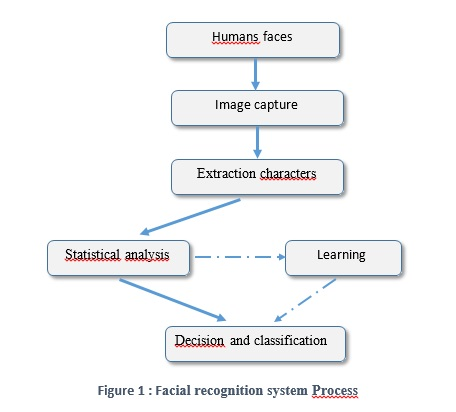
\includegraphics[scale=0.75]{fr_process}%[height=70mm,width=70mm]
\caption{\textbf{Facial recognition system process}}%
%\url {http://www.google.fr/}
\label{fr_process}%
\end {center}
\end{figure}

Facial recognition is facing the following problems:
\begin{itemize}
\item Change of pose ;
\item Light Variations ;
\item Variations of expression, age ;
\item Partial occultation of the face (concealing).
\end{itemize}

These variations are the most difficult because the variations in the appearance of a person face according to different pose or light conditions are often far more important than the variation between face images of two different individuals acquired under the same conditions.
This explains why pictures should be taken in specific conditions so that facial recognition can be efficient.

\subsection{The methods used for face recognition}	

Facial recognition methods can be classified into two broad categories: local and global methods. Amongst those methods, main ones will be presented thereafter.



\subsubsection{Global methods}

Global methods are based on well known techniques of statistical analysis. In these methods, face images (which can be shown as matrices of pixel values) are used as input of the recognition algorithm and are generally transformed into vectors, which are easier to handle. The main advantage of global methods is that they are relatively quick to set up in. However, they are very sensitive to variations of illumination, pose and facial expression.
\paragraph{}
The main existing methods are:
\begin{itemize}
\item The Principal Component Analysis (PCA) : EigenFaces
\item The LDA (Linear Discriminant Analysis) Algorithm : FisherFaces
\end{itemize}

\subsubsection{Local methods (Geometric)}

The local methods  include transformations applying to specific areas of the image, usually around characteristic points (corners of the eyes, mouth, nose, ...). Therefore, they require a priori knowledge on images. These methods are more difficult to implement but are more robust to the problems due to variations of illumination, pose and facial expression. The main existing methods are:
\begin{itemize}
\item EBGM (Elastic Bunch Graph Matching);
\item Modular Eigenface;
\item Hidden Markov Method.
\end{itemize}


But in fact, our aim on this project will be obviously to use both main global methods.

\paragraph{}

Both methods that we will present are using a common training algorithm steps that are :
\begin{itemize}
\item Preprocessing of training image set
\item Normalization and estimation of mean image
\item Use of PCA/ LDA
\end{itemize}

PCA/ LDA are statistical tools used to implement facial recognition method. For instance the use of PCA is divided into two steps :
\begin{itemize}
\item The determination of the input image weight from projecting input image into the face space and by multiplying the resulted vector to eigenfaces of the database.
\item A Comparison of results with metrics such as euclidian distance.
\end{itemize}


%%%%%%%%%%%%%%%%%%%%%%%%%%%%%%%%%%%%%%%%%%%%%%%%%%%%%
\section{Eigenfaces}
\subsection{Presentation of Eigenfaces}


	
The Eigenface approach began with a search for a low-dimensional representation of face images. Sirovich and Kirby in 1987 showed that Principal Component Analysis could be used on a collection of face images to form a set of basis features. These basis images, known as Eigenpictures, could be linearly combined to reconstruct images in the original training set.The approach of using eigenfaces for recognition was developed by Sirovich and Kirby and used by Matthew Turk and Alex Pentland in face classification.
Eigenfaces is the name given to a set of eigenvectors when they are used in the computer vision problem of human face recognition. The eigenvectors are derived from the covariance matrix of the probability distribution over the high-dimensional vector space of face images. The eigenfaces themselves form a basis set of all images used to construct the covariance matrix. This produces dimension reduction by allowing the smaller set of basis images to represent the original training images. Classification can be achieved by comparing how faces are represented by the basis set.

\subsection{Procedure}

A set of eigenfaces can be generated by performing a mathematical process called Principal Component Analysis (PCA) on a large set of images depicting different human faces. Informally, eigenfaces can be considered as a set of "standardized face ingredients", derived from statistical analysis of many pictures of faces. Any human face can be considered to be a combination of these standard faces.
\paragraph{}
To create a set of eigenfaces, one must:
\begin{itemize}
\item Prepare a training set of face images. The pictures constituting the training set should have been taken under the same lighting conditions, and must be normalized to have the eyes and mouths aligned across all images. They must also be all resampled to a common pixel resolution (r × c). Each image is treated as one vector, simply by concatenating the rows of pixels in the original image, resulting in a single row with r × c elements. For this implementation, it is assumed that all images of the training set are stored in a single matrix T,  where each column of the matrix is an image.
\item Calculate the average image by adding each columns of the matrix T and dividing the previous obtained vector by the number of input images.
\item Subtract the mean from matrix T to obtain matrix A (where each element represents the luminance variance of each pixel). Once the average image a is calculated and it is then subtracted from each original image in T.
\item Calculate the covariance matrix S.
\item Calculate the eigenvectors and eigenvalues of the covariance matrix S. Each eigenvector has the same dimensionality (number of components) as the original images, and thus can itself be seen as an image. The eigenvectors of this covariance matrix are therefore called eigenfaces. They are the directions in which the images differ from the mean image. Sort the eigenvalues in descending order and arrange eigenvectors accordingly.
\item Choose the principal components. The number of principal components k is determined arbitrarily by setting a threshold ε on the total variance.
Total variance v = n*(λ1+ λ2+…+ λn), n= number of data images.
\item k is the smallest number satisfies.
\item Determinate the input image weight determination from projecting each image.
\item Each image is represented by a vector which is used to reconstruct the images. We then save the average image, eigenfaces and the projection (weight ) of images.
\end{itemize}


This ends the training part of the implementation of eigenfces and shows the skills used.



\paragraph{EigenFaces logigram }

The flowchart we  have to use is  divided into two basic parts: the learning phase and the identification phase where the Euclidean distance is used to calculate the difference between the weight of the image to be identified and the database images, then the program displays the nearest.
\paragraph{}
But retain before these two major steps,we have  pretreatments and it’s the phase which is carried out :
\begin{itemize}
\item The selection of the learning base ;
\item Reading images ;
\item The conversion of grayscale images ;
\item Resizing images ;
\item And finally the application of histogram equalization.
\end{itemize}


\begin{figure}[bth]%[!ht]
\begin{center}
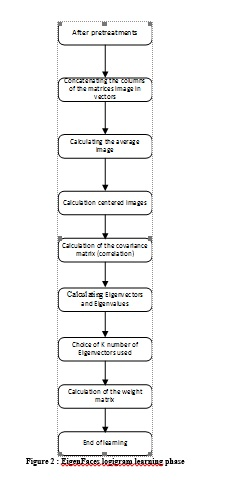
\includegraphics[scale=0.75]{ef_learningphase}%[height=70mm,width=70mm]
\caption{\textbf{EigenFaces logigram learning phase}}%
%\url {http://www.google.fr/}
\label{ef_learningphase}%
\end {center}
\end{figure}	


\begin{figure}[bth]%[!ht]
\begin{center}
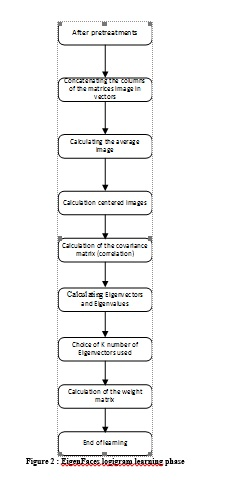
\includegraphics[scale=0.75]{ef_learningphase}%[height=70mm,width=70mm]
\caption{\textbf{EigenFaces logigram identification phase}}%
%\url {http://www.google.fr/}
\label{ef_idphase}%
\end {center}
\end{figure}	

\subsection{Benefits and deficiencies}	
\subsubsection{Benefits}	
Eigenface provides an easy and cheap way to realize face recognition in that:
\begin{itemize}
\item Its training process is completely automatic and easy to code. 
\item Eigenface adequately reduces statistical complexity in face image representation.
\item Once eigenfaces of a database are calculated, face recognition can be achieved in real time.
\item Eigenface can handle large databases.
\end{itemize}


\subsubsection{Deficiencies}
However, the deficiencies of the eigenface method are also obvious:
\begin{itemize}
\item Very sensitive to lighting, scale and translation; requires a highly controlled environment.
\item Eigenface has difficulty capturing expression changes.
\item 
\item 
\end{itemize}

The most significant eigenfaces are mainly about illumination encoding and don't provide useful information regarding the actual face.






%%%%%%%%%%%%%%%%%%%%%%%%%%%%%%%%%%%%%%%%%%%%%%%%%%%%%
\section{Fisherfaces}
\subsection{•}
\subsubsection{•}
\begin{itemize}
\item Very sensitive to lighting, scale and translation; requires a highly controlled environment.
\item Eigenface has difficulty capturing expression changes.
\item 
\item 
\end{itemize}











\paragraph{} On souhaite dans cette partie transmettre un fichier binaire quelconque sur la chaîne de transmission.

\paragraph{} Soit un fichier texte avec le nom "Thomas Le Bris" dedans, son code ASCII en décimal sera :\begin{description}
\item[84 104 111 109 97 32 76 101  32 66 114 105 115]
\end{description}

\paragraph{} En ouvrant le fichier dans Matlab à l'aide de la fonction précédente nous obtenons bien le code prévu :

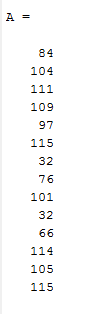
\includegraphics[scale=1]{ASCIInom.PNG}

\paragraph{} Pour obtenir le code ASCII il nous suffit d'écrire Master 1 RTMA dans le fichier texte puis de l'ouvrir dans Matlab :
\newline
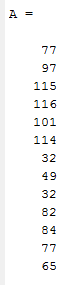
\includegraphics[scale=1]{ASCIIrtma.PNG}

\paragraph{} ADS nécessitant un fichier texte ne comportant que des '0' et '1' formatés en une seul colonne Nous allons utiliser Matlab afin d'effectuer la conversion d'un fichier texte en binaire puis son formatage approprié.

\begin{description}
\item[cf fichier joint conv2ADS.m]
\end{description}

 
\paragraph{} ADS nous renvoyant en sortie un fichier formaté de la même façon il nous réutiliserons Matlab afin de reconvertir le fichier traité par la chaîne de transmission dans son format original.

\begin{description}
\item[cf fichier joint ADS2ASCII.m]
\end{description} 

\paragraph{} En transmettant le fichier dans des conditions favorables nous obtenons bien un fichier identique mais en augmentant le bruit des erreurs apparaissent sur le fichier en sortie :
\begin{figure}[h]
  \centering
  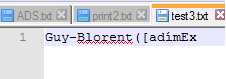
\includegraphics{erreur_txt_teb_0_0057.png}
  \caption{TEB = 0.0057}
\end{figure}



\paragraph{}Jusqu'à devenir complètement différent du fichier original avec un TEB égal à 0.5 :
\begin{figure}[h]
  \centering
 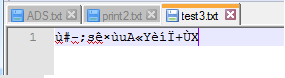
\includegraphics{erreur_txt_teb_0_5.png}
  \caption{TEB = 0.5}
\end{figure}


\paragraph{} Cela est dû au fait que le bruit transforme des 0 en 1 et des 1 en 0 ce qui fausse donc la conversion lors du retour en ASCII.
 
 
 
 
 
 














































 
 
 
 
 
 
 
 
 




	%\chapter{Tableau de synthèse des résultats obtenus}
\minitoc

\begin{tabular}{|c|c|c|c|}
\hline 
 & JPEG & BMP & MP4 \\ 
\hline 
fichier original & 
\includegraphics{test_jpeg.jpg} & 
\includegraphics{test.png} & 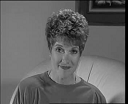
\includegraphics{vlcsnap-origine.png} \\ 
\hline 
$TEB_1$ & 2.8E-5 & 1.5E-4 & 2.1E-5 \\ 
\hline 
$TEB_2$ & 1.5E-4 & 0.001 & 0.004 \\ 
\hline 
$TEB_1<TEB<TEB_2$ & 
\includegraphics{jpg_test_bruit63dB.jpg} & 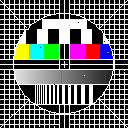
\includegraphics{BMP_test_bruit62dB.png} & 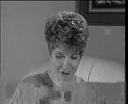
\includegraphics{vlcsnap-bruit.png} \\ 
\hline 
Robuste ? & non & oui & non \\ 
\hline 
Type d'erreurs constatées & Effets blocs, désynchronisation & Erreurs pixels & Effets blocs, désynchronisation \\ 
\hline 
\end{tabular} 
	%\include{Partie5}
	%\chapter*{Conclusion}
\addcontentsline{toc}{chapter}{Conclusion}
\minitoc


A l'issu de cette séance, nous avons une meilleure vision de la caractérisation d'un fichier et de la transmission des données sur une chaine de transmission.
\paragraph{}
Ceci est un plus en terme de compétences à notre formation, en ce sens que nous apprenons par ces travaux à caractériser les données numériques qui sont binaires et mieux connaitre les formats et les erreurs inhérentes.


	
 % \appendix

	
  %\include{Annexe}
	
 	\bibliographystyle{alpha} %classe les entrées par ordre alphabétique et les numérote en conséquence 

	\bibliography{biblio}
	
\end{document}

%Fin Redaction du document
%%%%%%%%%%%%%%%%%%%%%%%%%%%%%%%%%%%%%%%%%%%%%%%%%%%%%%%%%%%%%%%%%%%%%%%%%%%%%%%%%%%%%%